%-------------------3.1
\subsection{Code listing using \textit{\fbox{minted}} in \mybox[red]{beamer}}
\begin{table}[h!]
\begin{tabular}{c | c}
\begin{minipage}[m]{0.4\textwidth}
\enum{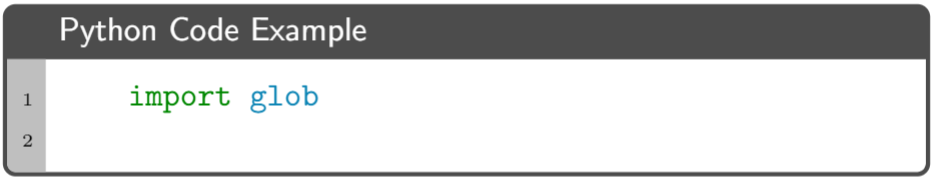
\includegraphics[width=1\linewidth]{3.1.png}}{3.1}
\end{minipage}
&
\begin{minipage}[m]{0.55\textwidth}
\renewcommand\textminus{\mbox{-}}%<<<<<<<<<<<
\begin{lstlisting}[numberstyle=\zebra{pink!15}{green!15},numbers=left,basicstyle=\ttfamily\footnotesize]{tex}
\documentclass{beamer}
\usepackage{tcolorbox}
\tcbuselibrary{minted,skins,breakable}
\newtcblisting{pythoncode}[2][]{
  listing engine=minted, breakable,  colback=bg,
  colframe=black!70,  listing only,
  minted style=colorful,  minted language=python,
  minted options={numbersep=3mm,texcl=true,#1},
  left=5mm,enhanced,
  overlay={\begin{tcbclipinterior}\fill[black!25] (frame.south west)
rectangle ([xshift=5mm]frame.north west);\end{tcbclipinterior}},
#2,}
\begin{document}
\begin{frame}[fragile]
    \frametitle{Premature Optimization}
    \begin{pythoncode}[linenos=true,]{title=Python Code Example}
    import glob
    \end{pythoncode}
\end{frame}
\end{document}
\end{lstlisting}
\end{minipage}
\end{tabular}
\end{table}

%-------------------3.2
\subsection{"Zebra" style listing}
\begin{table}[h!]
\begin{tabular}{c | c}
\begin{minipage}[m]{0.4\textwidth}
 \begin{lstlisting}[numberstyle=\zebra{green!25}{yellow!25},numbers=left,basicstyle=\ttfamily\footnotesize]
/**
* Prints Hello World.
**/
#include <stdio.h>

int main(void) {
   printf("Hello World!");
   return 0;
}
\end{lstlisting} 
\end{minipage}
&
\begin{minipage}[m]{0.55\textwidth}
\renewcommand\textminus{\mbox{-}}%<<<<<<<<<<<
\begin{tiny}
\begin{verbatim}
\documentclass{article}
\usepackage[T1]{fontenc}
\usepackage{beramono}
\usepackage{listings}
\usepackage{xcolor}
\newcommand\realnumberstyle[1]{}
\makeatletter
\newcommand{\zebra}[3]{%
    {\realnumberstyle{#3}}%
    \begingroup
    \lst@basicstyle
    \ifodd\value{lstnumber}%
        \color{#1}%
    \else
        \color{#2}%
    \fi
        \rlap{\hspace*{\lst@numbersep}%
        \color@block{\linewidth}{\ht\strutbox}{\dp\strutbox}%
        }%
    \endgroup}
\makeatother
\begin{document}
\begin{lstlisting}[language=C,basicstyle=\ttfamily,
numberstyle=\zebra{green!35}{yellow!35},numbers=left]
/**
* Prints Hello World.
**/
#include <stdio.h>
int main(void) {
   printf("Hello World!");
   return 0;
}
\end{lstlisting}
\end{document}
\end{verbatim}
\end{tiny}
\end{minipage}
\end{tabular}
\end{table}
\clearpage

%-------------------3.3

\subsection{Listing with russian language}
\begin{table}[h!]
\begin{tabular}{c | c}
\begin{minipage}[m]{0.4\textwidth}
\enum{ 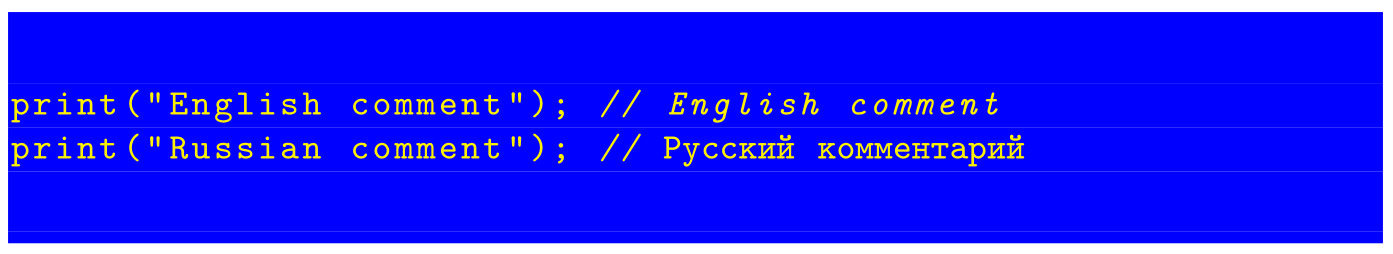
\includegraphics[width=1\linewidth]{3.3.png} }{3.3}
\end{minipage}
&
\begin{minipage}[m]{0.55\textwidth}
\renewcommand\textminus{\mbox{-}}%<<<<<<<<<<<
\begin{lstlisting}[numberstyle=\zebra{pink!15}{green!15},numbers=left,basicstyle=\ttfamily\footnotesize] 
\documentclass{article}
\usepackage[T2A]{fontenc}
\usepackage[utf8]{inputenc}
\usepackage[russian]{babel}
\usepackage{listings} 
\usepackage{xcolor}

\begin{document}
\lstset{ keepspaces=true, 
backgroundcolor=\color{blue},  
showstringspaces=false, 
language=C, 
extendedchars=\true, 
framexrightmargin=0pt,
framexleftmargin=0pt,
framextopmargin=15pt,
framexbottommargin=15pt, 
frame=tb, framerule=0pt,
basicstyle=\color{yellow}\ttfamily\small}

begin{lstlisting}% <<<<<<<<< add "/"
print("English comment"); // English comment
print("Russian comment"); // %here can be russian words
end{lstlisting}%   <<<<<<<<< add "/"
\end{document}
\end{lstlisting}
\end{minipage}
\end{tabular}
\end{table}
 
%-------------------3.4

\subsection{Listing with \texttt{\fbox{minted}}}
\begin{table}[h!]
\begin{tabular}{c | c}
\begin{minipage}[m]{0.4\textwidth}
\enum{ \href{https://tex.stackexchange.com/questions/174455/typeset-source-code-with-tcolorbox}{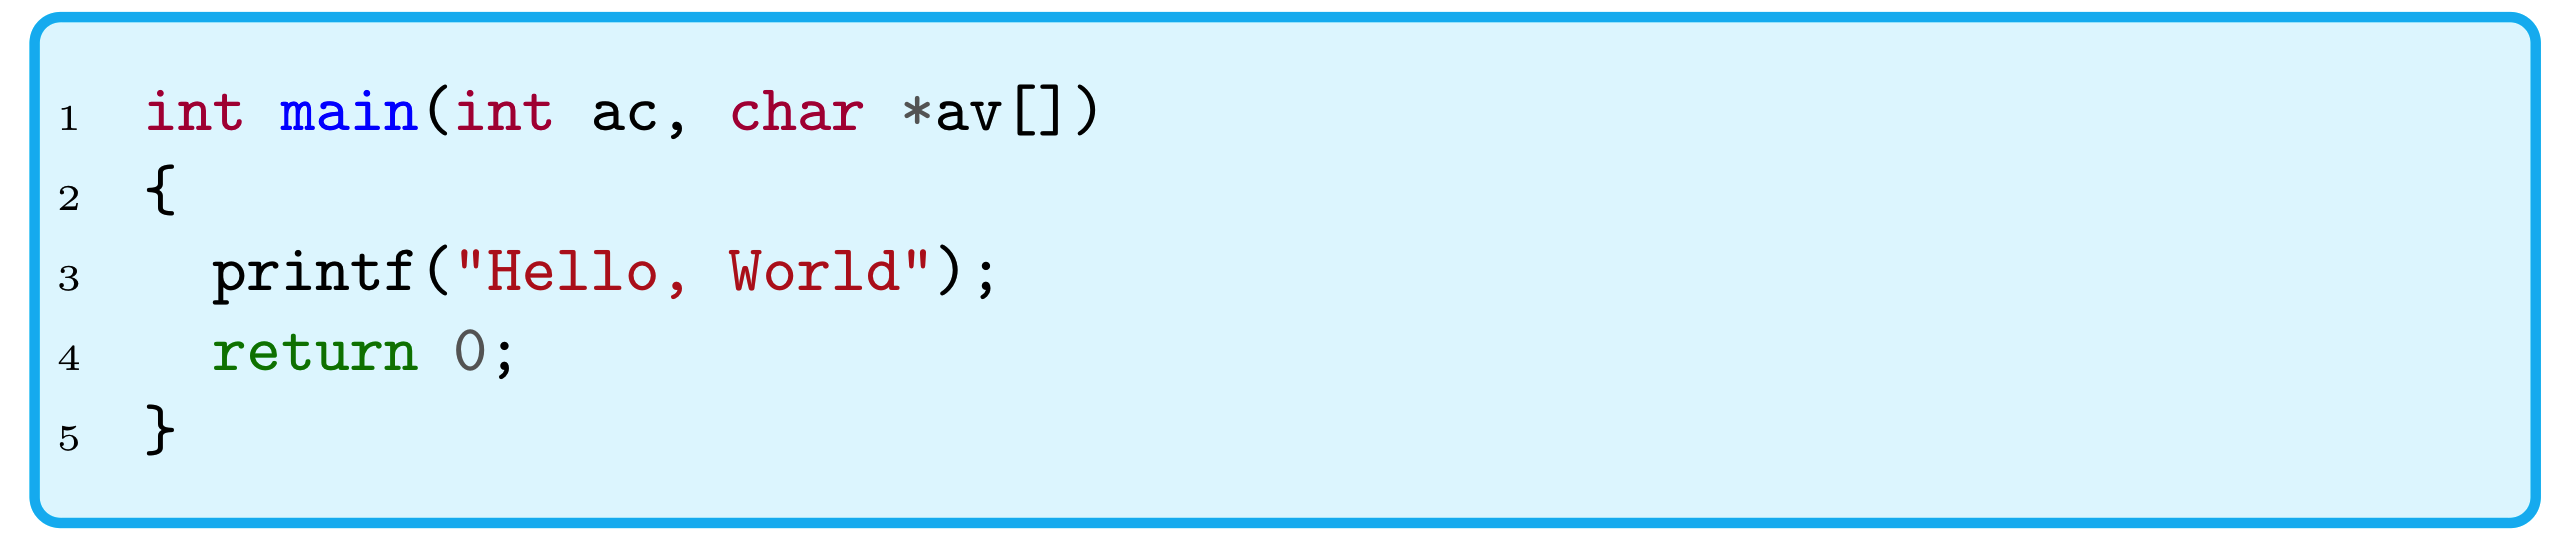
\includegraphics[width=1\linewidth]{3.4.png}} }{3.4}
\end{minipage}
&
\begin{minipage}[m]{0.55\textwidth}
\renewcommand\textminus{\mbox{-}}%<<<<<<<<<<<
\begin{lstlisting}[numberstyle=\zebra{pink!15}{green!15},numbers=left,basicstyle=\ttfamily\footnotesize] 
\documentclass{article}
\usepackage[many]{tcolorbox}
\tcbuselibrary{minted}
\newtcblisting{mylisting}{
  colframe=cyan,
  colback=cyan!10,
  listing only,
  listing engine=minted,
  minted language=cpp,
  minted options={fontsize=\small,linenos,numbersep=3mm},
}

\begin{document}
\begin{mylisting}
some code 
\end{mylisting}
\end{document}
\end{lstlisting}
\end{minipage}
\end{tabular}
\end{table}
%-------------------3.5
%-------------------3.6
%-------------------3.7
%-------------------3.8
%-------------------3.9
%-------------------3.10









